In this problem, we draw the block diagram of the linearised loudspeaker (see figure \ref{fig:linearModel}) showing the couplings between the different states.

\begin{figure}[H]
 \centering 
 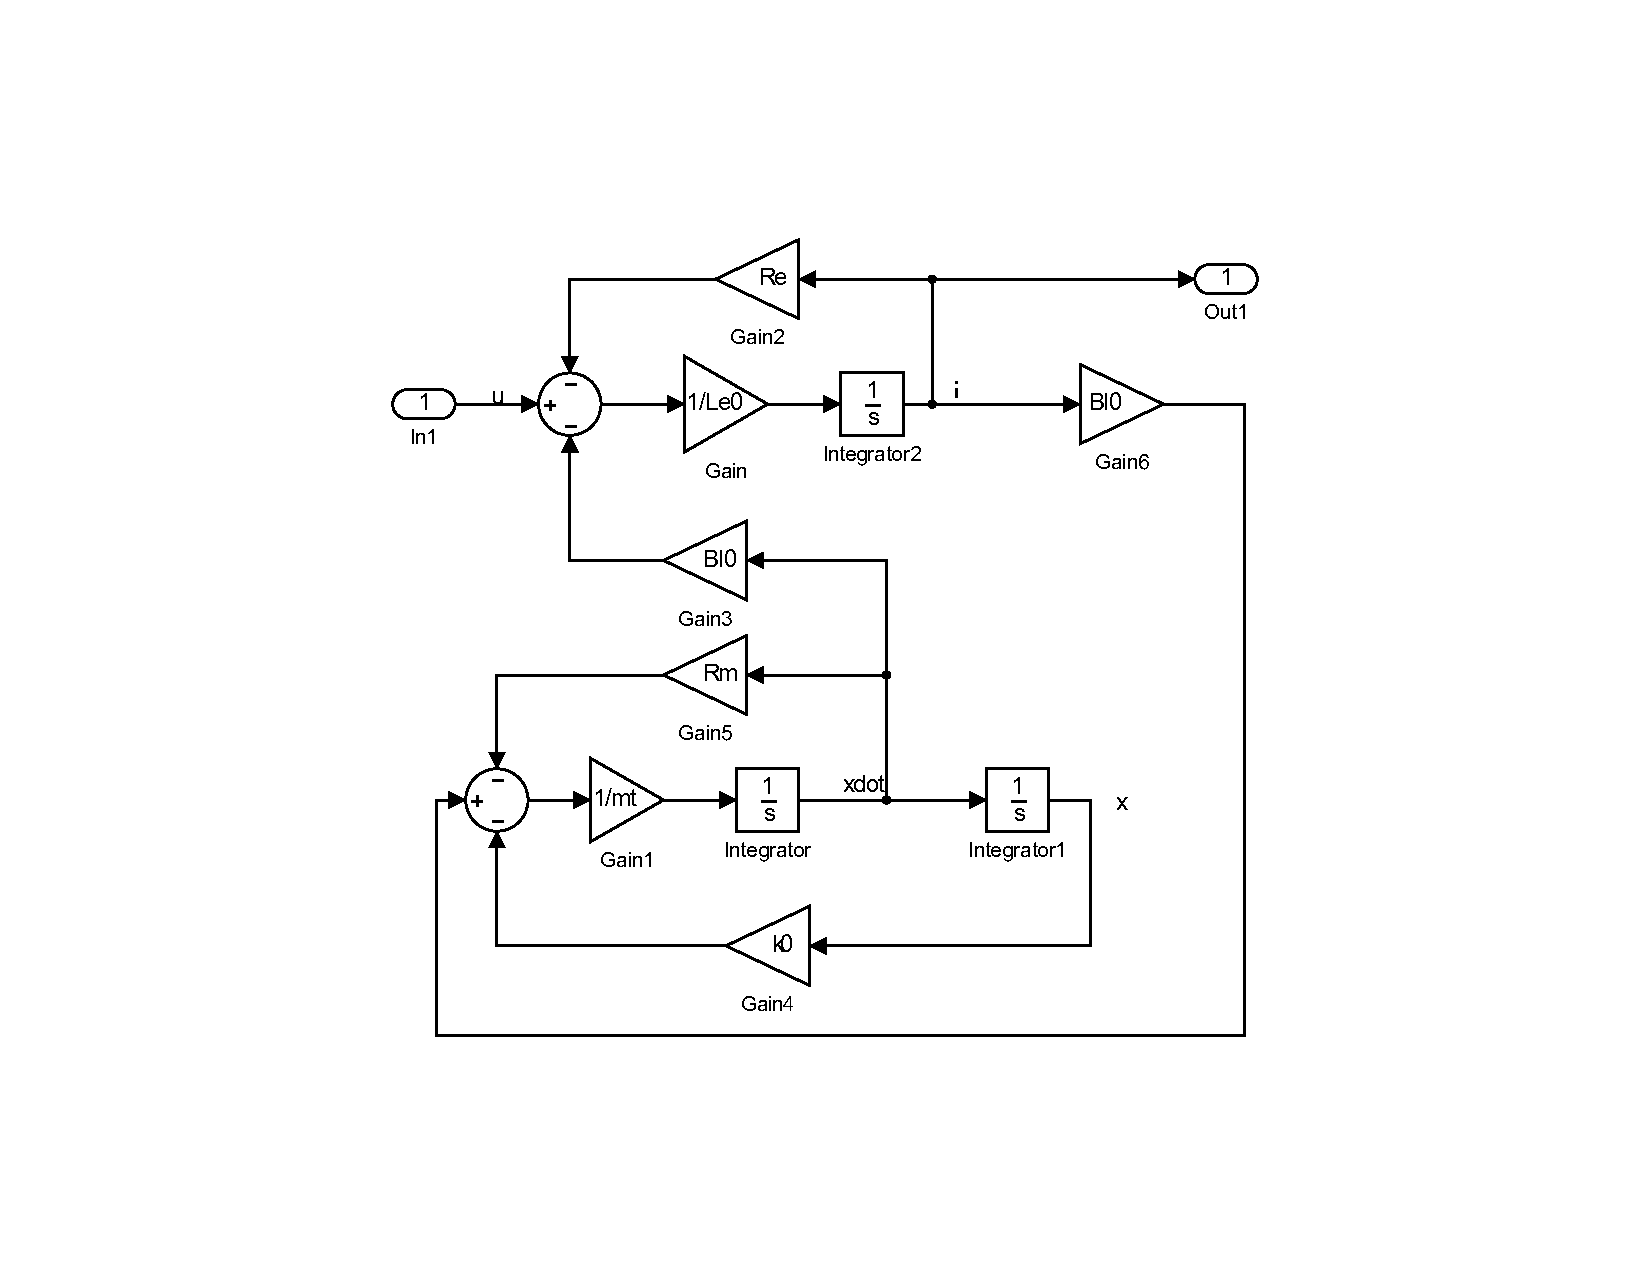
\includegraphics[trim=5cm 3cm 2cm 3cm, clip=true, totalheight=0.5\textheight, angle=0]{figures/linearModel.pdf}
 \caption{block diagram of the linearised loudspeaker}
\label{fig:linearModel}
\end{figure}

By means of this block diagram, we can make preliminary assessments of the system. Indeed, we can see that the state $i$ seems to be controllable and observable as it is connected to the input $u_e$ and to the output. However, the states $x$ and $\dot{x}$ seems to be controllable as they are also connected to the input $u_e$ but not to be observable because they are not connected to any output. Moreover the 3 states seems to be stable because of the 2 backloops.

We can verify our assumptions regarding the controllability and the observability by calculating the $rank$ of $M_c$ and $M_o$.
\begin{lstlisting}[language=Matlab]
Mc = [B A*B A^2*B];
rank(Mc) % = 3 controllable
Mo=[C
    C*A
    C*A^2];
rank(Mo) % = 3 observable
\end{lstlisting}


